
In section \ref{Sec:Motion Data} we discuss our experiment with both the iPhone and Wrist Monitor mounted on the same hand.
This experiment

Some of the characteristic movements and their resultant noticable signals are shown in table \ref{Tab:Signals}.

% Please add the following required packages to your document preamble:
% \usepackage{booktabs}
\begin{table}[h]
\centering
\resizebox{0.8\textwidth}{!}{%
\begin{tabular}{@{}lll@{}}
\toprule
Description of movement       & Photograph of movement 									      & Select identifiable signal in WristView\\ \midrule
Move Hand up and down         & \parbox[c]{2in}{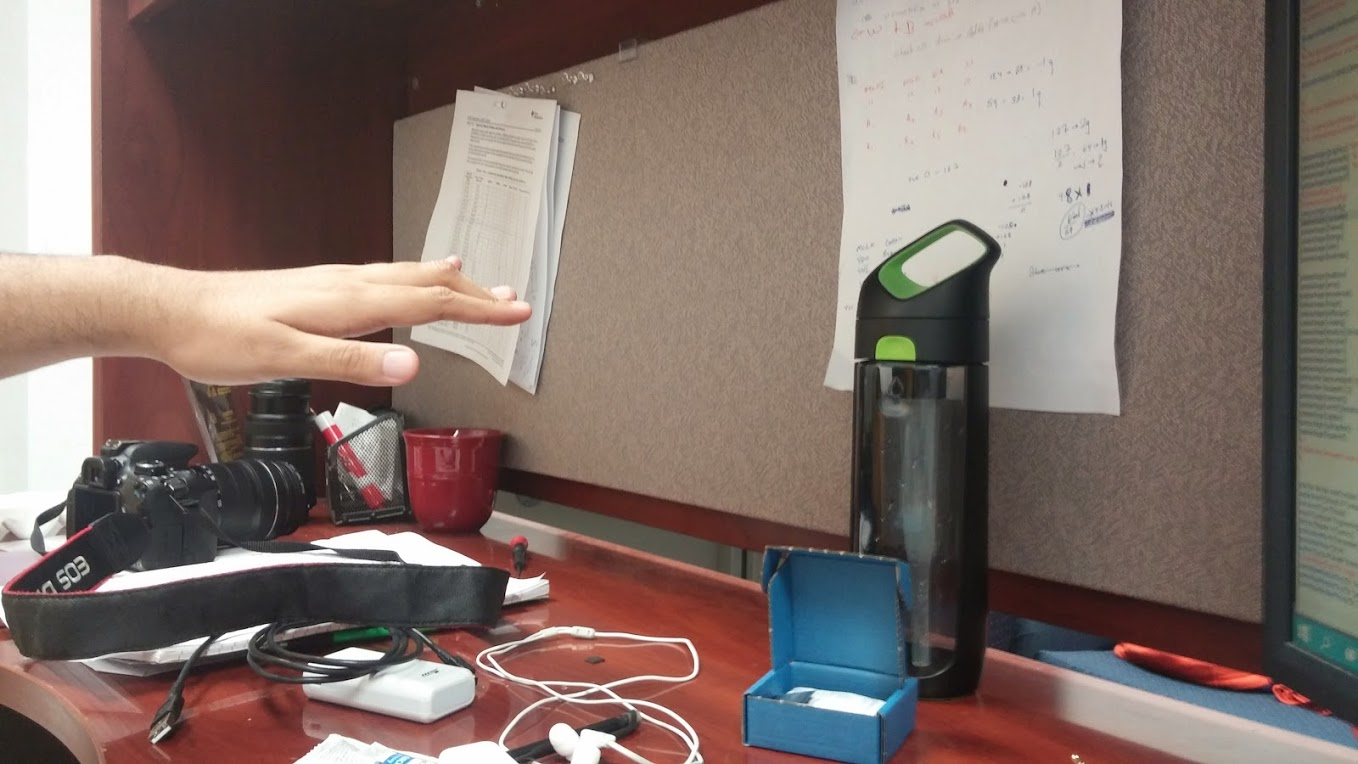
\includegraphics[width=2in]{images/HandMovement}\\[2ex]} & \parbox[c]{1in}{~~~~~~~~~~~~~~~~~~ 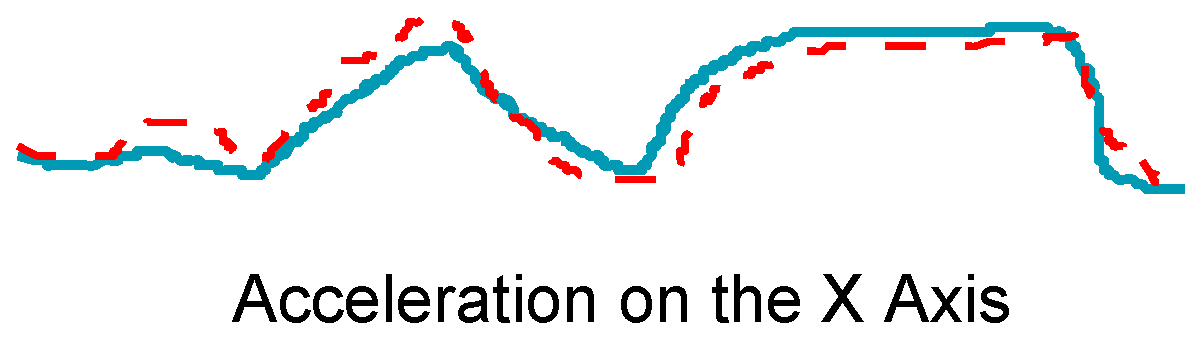
\includegraphics[width=1in]{images/RandomSignal.eps}} \\ 
Rotate Hand Clockwise         & \parbox[c]{2in}{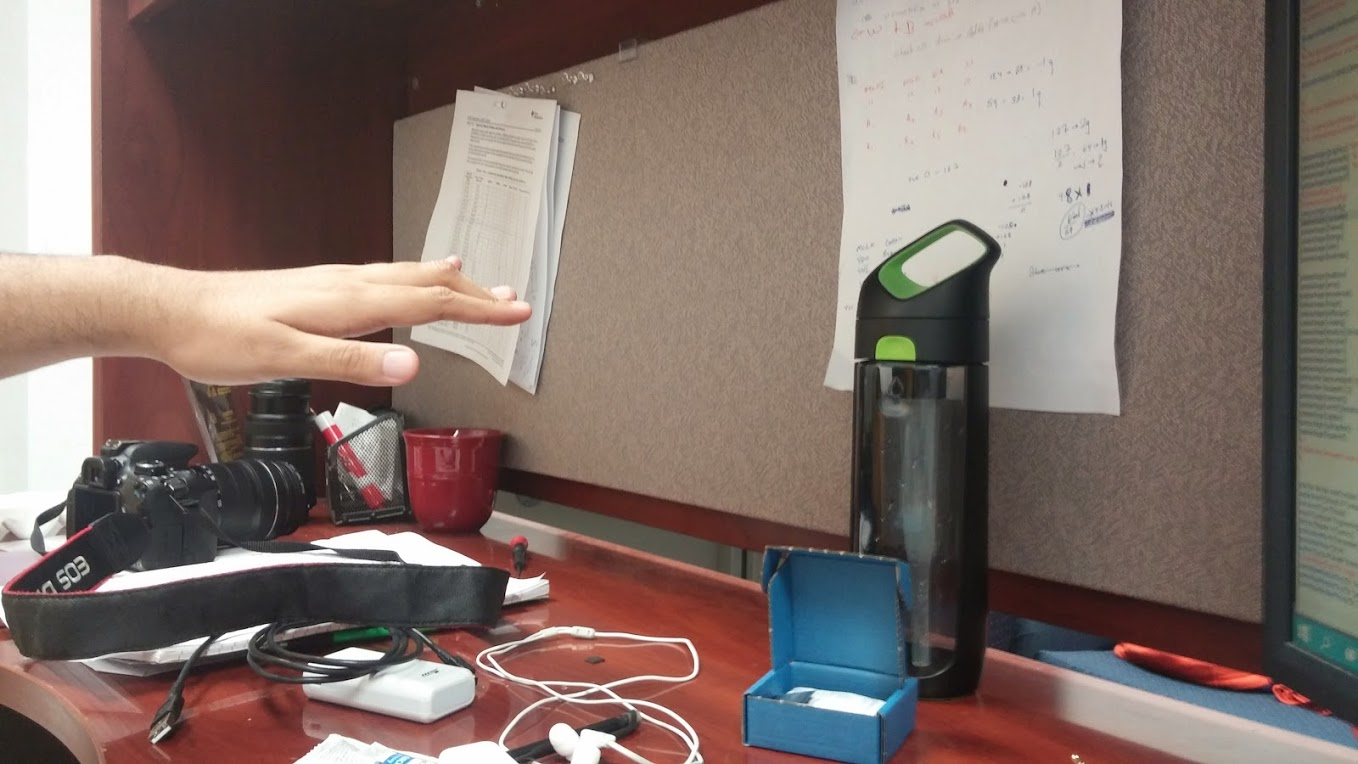
\includegraphics[width=2in]{images/HandMovement}\\[2ex]} & \parbox[c]{1in}{~~~~~~~~~~~~~~~~~~ 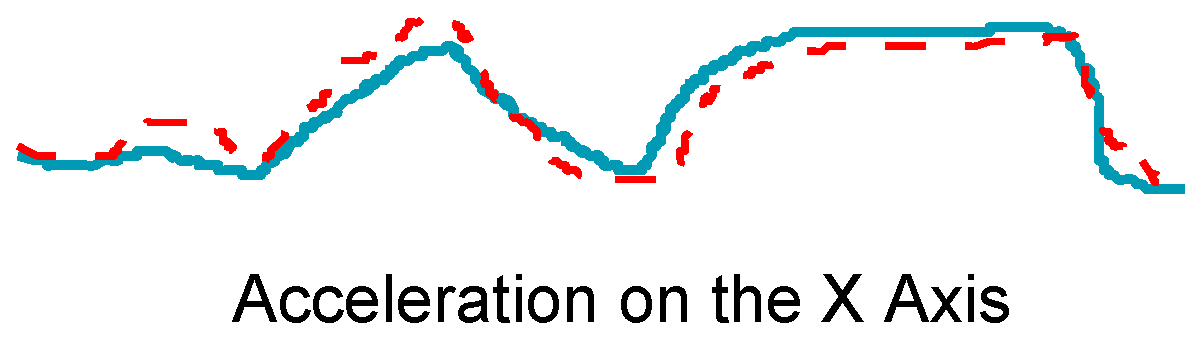
\includegraphics[width=1in]{images/RandomSignal.eps}} \\ 
Rotate Hand Counter Clockwise & \parbox[c]{2in}{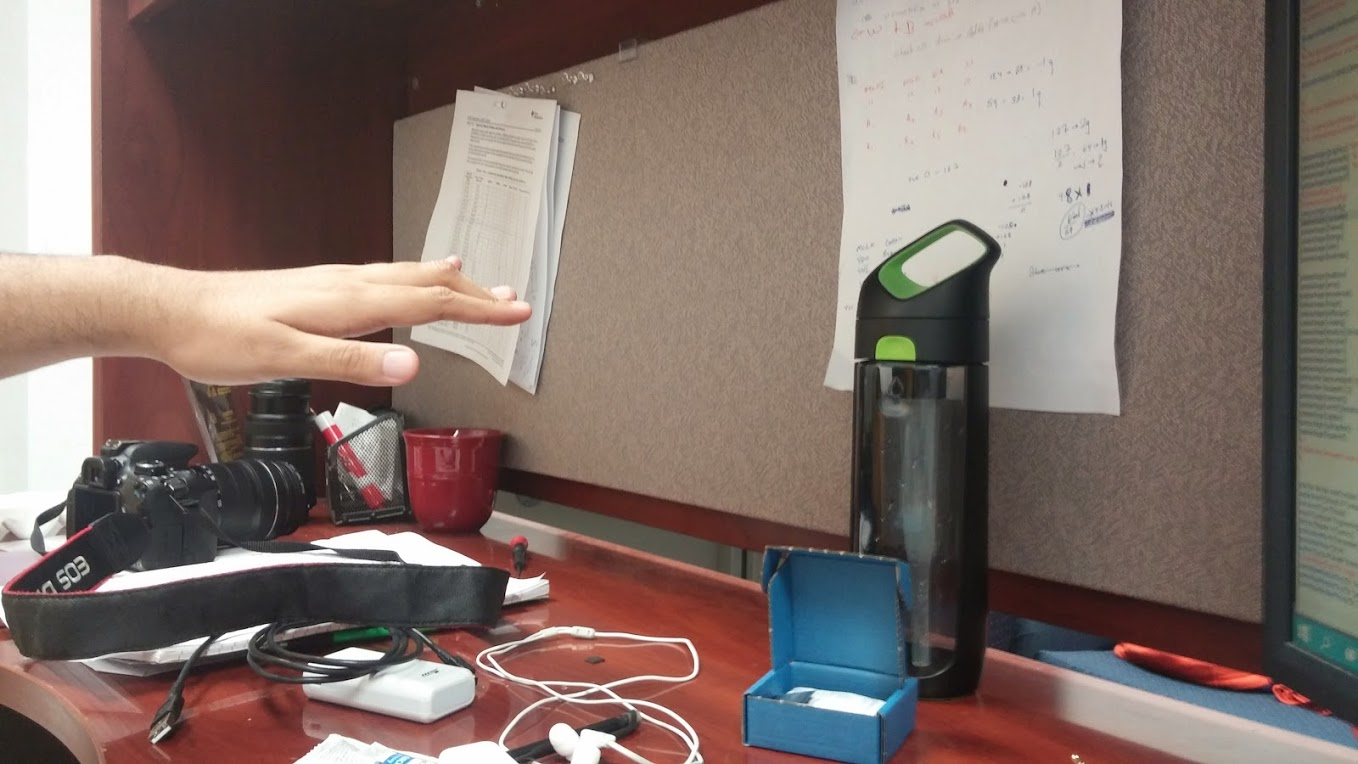
\includegraphics[width=2in]{images/HandMovement}\\[2ex]} & \parbox[c]{1in}{~~~~~~~~~~~~~~~~~~ 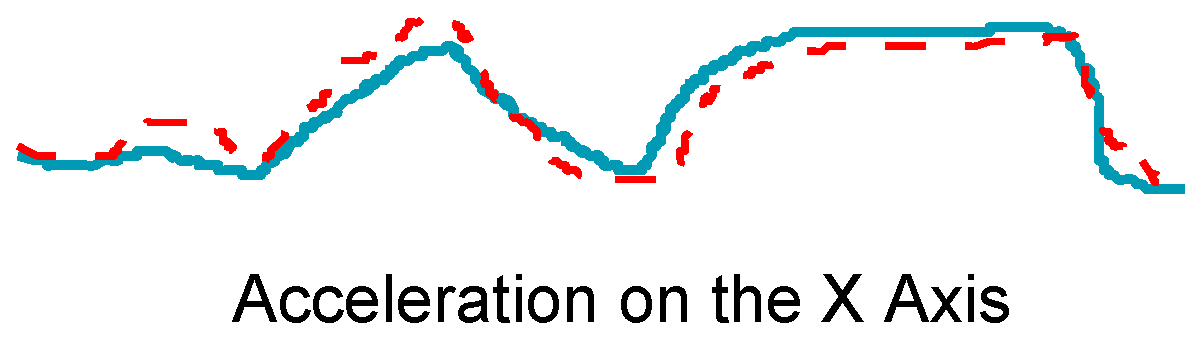
\includegraphics[width=1in]{images/RandomSignal.eps}} \\ 
Move Device to the left.      & \parbox[c]{2in}{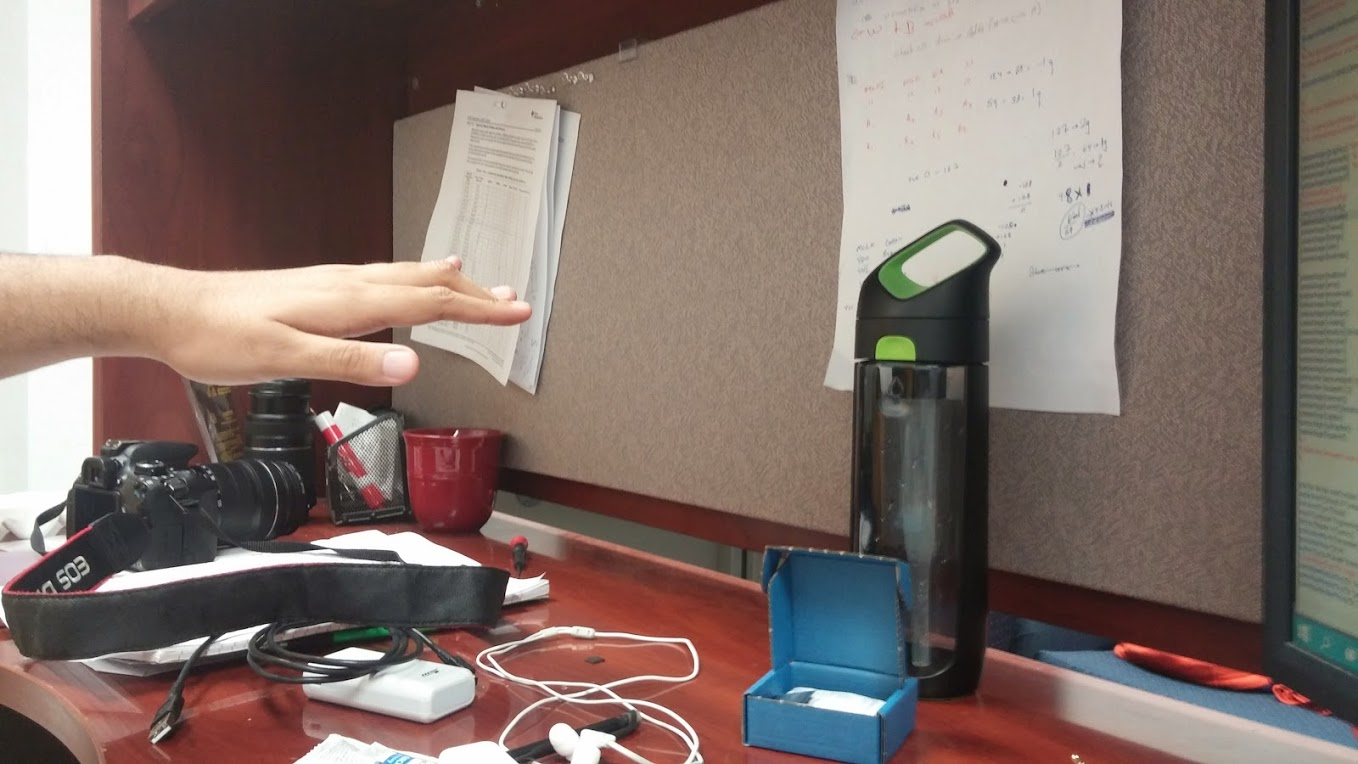
\includegraphics[width=2in]{images/HandMovement}\\[2ex]} & \parbox[c]{1in}{~~~~~~~~~~~~~~~~~~ 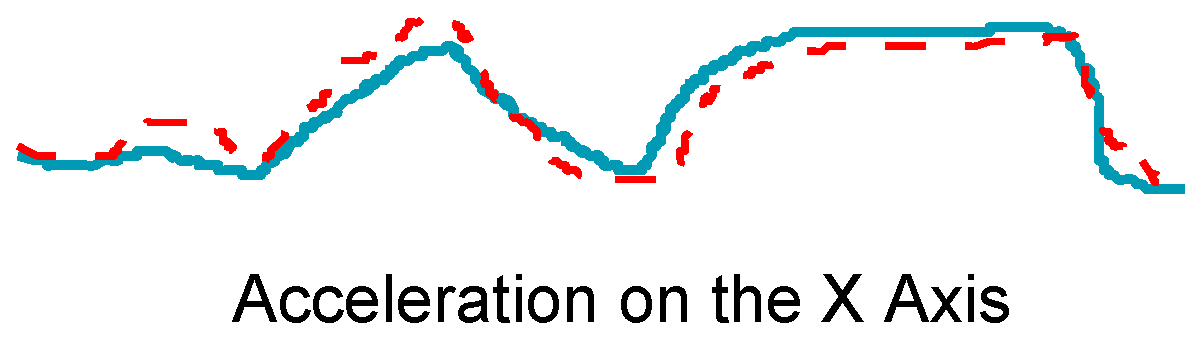
\includegraphics[width=1in]{images/RandomSignal.eps}} \\ 
Move Device forward.          & \parbox[c]{2in}{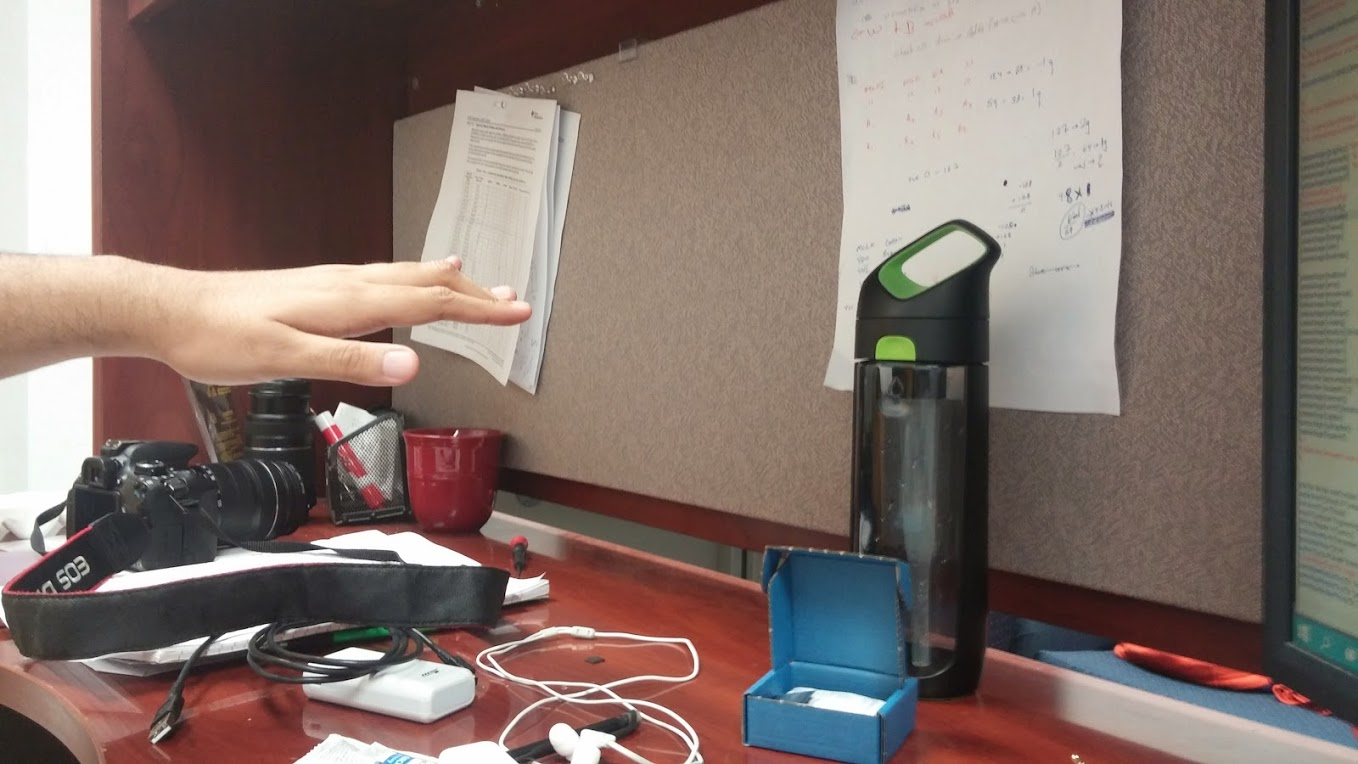
\includegraphics[width=2in]{images/HandMovement}\\[2ex]} & \parbox[c]{1in}{~~~~~~~~~~~~~~~~~~ 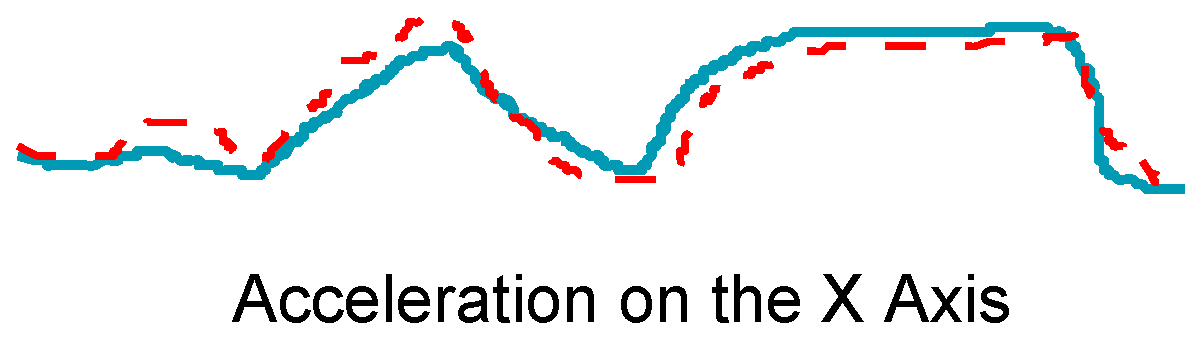
\includegraphics[width=1in]{images/RandomSignal.eps}} \\ 
Move Device to the right.     & \parbox[c]{2in}{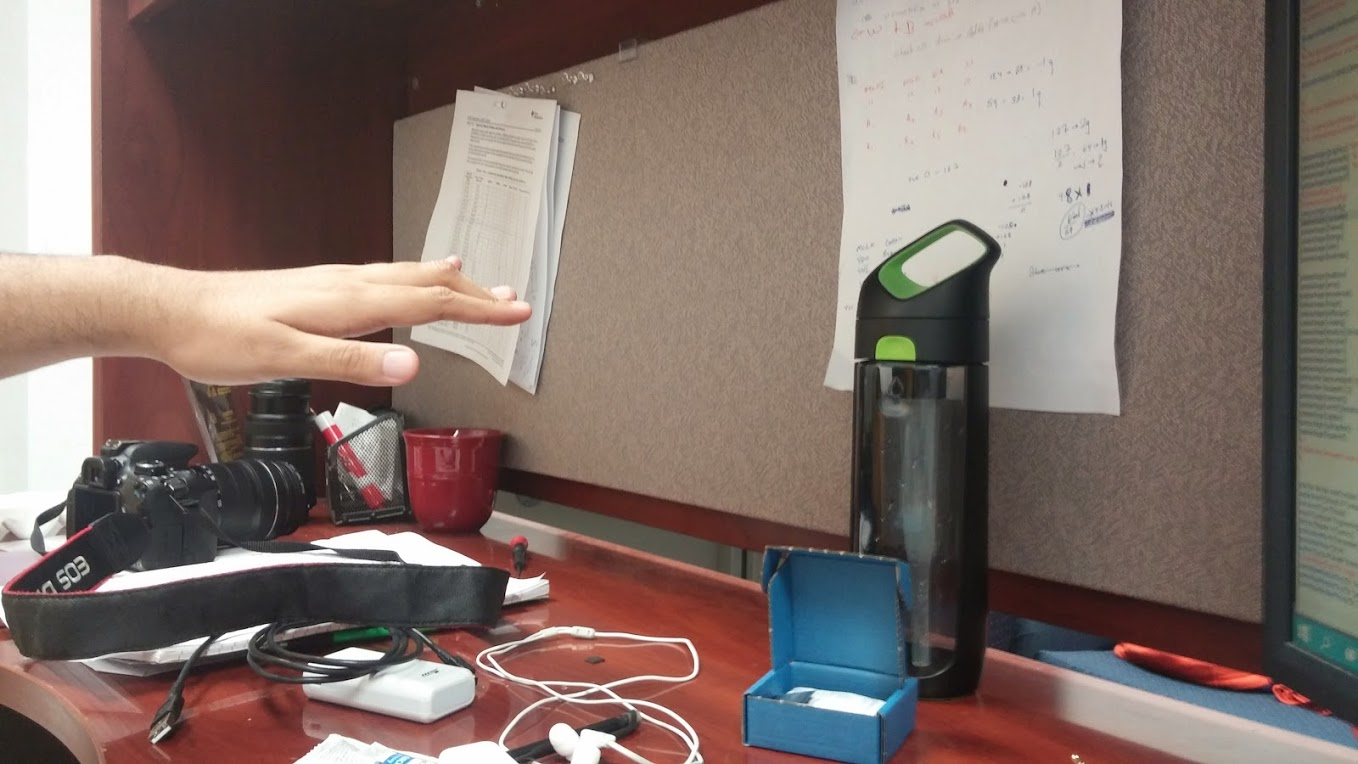
\includegraphics[width=2in]{images/HandMovement}\\[2ex]} & \parbox[c]{1in}{~~~~~~~~~~~~~~~~~~ 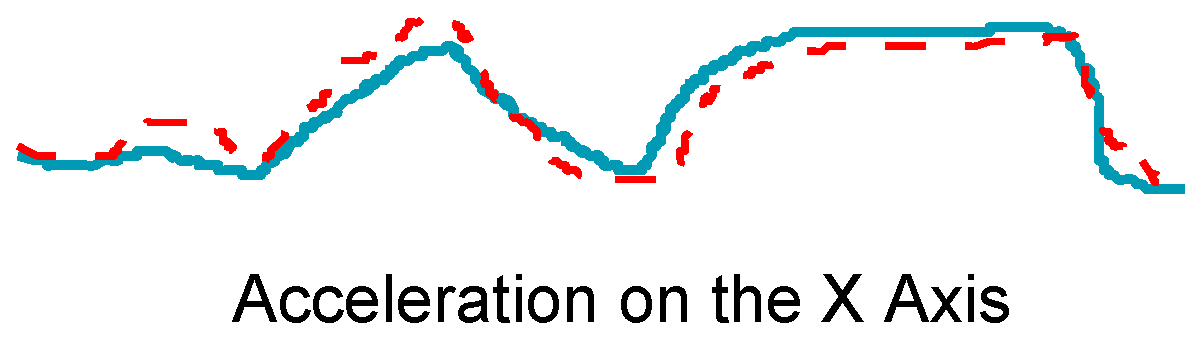
\includegraphics[width=1in]{images/RandomSignal.eps}} \\ \bottomrule
 
\end{tabular}
}
\caption{Different characteristic movements tested with an iPhone (red dashes) and our device (blue solid)}
\label{my-label}
\end{table}

\section{Comfort Analysis}
\label{Sec:Comfort}

Table \ref{Tab:Comfort} shows the list of periods worn by each user,
and the rating they provided us with after the experiment.

\section{Device Comparison}
\label{Sec:Comparison}
As mentioned in the Introduction (\ref{Chap:Intro}),
multiple devices exist in the market that might perform features similar to our Wrist motion activity tracker.
Table \ref{Tab:Comparison} compares these devices.

\chapter{Conclusion and Future Work}

